
\documentclass{article} % For LaTeX2e
\usepackage[accepted]{colm2026_conference}

\usepackage{microtype}
\usepackage{hyperref}
\usepackage{url}
\usepackage{booktabs}
\usepackage{multirow}
\usepackage{graphicx}
\usepackage{float}
\usepackage{placeins}
\usepackage{array}
% NOTE: including geometry package
% The geometery package modifies some page properties when used. This can dramatically change the page margins, leading to severe template violation, and potential desk rejection. If the package is required, it can be used with the "pass" flag to skip the default page modifications, as in the following line:
% \usepackage[pass]{geometry}

\usepackage{lineno}

\definecolor{darkblue}{rgb}{0, 0, 0.5}
\hypersetup{colorlinks=true, citecolor=darkblue, linkcolor=darkblue, urlcolor=darkblue}


\title{Why Does Multilingual Training Improve Theorem Proving? \\ A Small-Scale Controlled Study}

% Authors must not appear in the submitted version. This should be be taken care of automatically as long as you are using the "submission" option for the colm2026_conference package. But it's on the authors to verify. Non-anonymous submissions will be rejected without review.

\author{
Amadeo De La Vega \\
Department of Computer Science\\
University of Maryland
\And
Mehak Gupta \\
Department of Computer Science\\
University of Maryland
\And
Huan Zhou \\
Department of Civil and Environmental Engineering\\
University of Maryland\\
College Park, MD 20742, USA\\
\texttt{\{adelaveg,mgupta25,hzhou715\}@umd.edu}
}

% The \author macro works with any number of authors. There are two commands
% used to separate the names and addresses of multiple authors: \And and \AND.
%
% Using \And between authors leaves it to \LaTeX{} to determine where to break
% the lines. Using \AND forces a linebreak at that point. So, if \LaTeX{}
% puts 3 of 4 authors names on the first line, and the last on the second
% line, try using \AND instead of \And before the third author name.

\newcommand{\fix}{\marginpar{FIX}}
\newcommand{\new}{\marginpar{NEW}}

\begin{document}


\linenumbers


\maketitle
\nolinenumbers % For deleting line numbering

\begin{abstract}
Multilingual theorem-proving models can outperform monolingual baselines, but the reason is unclear.  Do models learn proof patterns shared by Lean and Rocq, or do they mainly benefit from seeing more syntax variation during training?  We study this question with three controlled CodeT5-small models in the ProofWala setting: E1, a Lean-only baseline; E3, a real multilingual Lean+Rocq model; and E4, a pseudo-multilingual Lean model built with meaning-preserving syntax changes.  We evaluate all models with the same proof-search pipeline on two Lean benchmarks.  On \textbf{Easy\_Lean}, E4 performs best (63.6\% pass rate, versus 38.6\% for E1 and 30.5\% for E3).  On \textbf{Hard\_Lean}, E3 performs best (4.9\%, versus 2.6\% for E1 and 3.4\% for E4).  The main finding is distribution-dependent: syntax variation helps most on Easy\_Lean, while real multilingual training helps most on Hard\_Lean.
\end{abstract}

\section{Problem Statement, Motivation, and Approach}

Recent neural theorem provers typically train a language model to map a proof state to the next tactic, then use the model inside a search procedure.  ProofWala reports that multilingual training across Lean and Rocq improves proof-search success~\citep{thakur2025proofwala}.  The open question is why.  We study two hypotheses.  \textbf{H1, cross-language transfer}, says that models learn proof patterns that transfer across proof assistants.  \textbf{H2, regularization}, says that syntax variation improves robustness by discouraging overfitting to language-specific syntax.

This project asks:

\begin{quote}
\textbf{When does multilingual training improve Lean proof search, and is the gain due to cross-system transfer or regularization?}
\end{quote}

We compare three models that differ only in training data.  E1 is trained on Lean proof steps only.  E3 is trained on real multilingual Lean+Rocq data.  E4 is trained on Lean plus a pseudo-Lean variant created by consistently renaming local variables and hypotheses.  E4 is the key control: it adds syntax variation without adding Rocq syntax, tactics, or libraries.  Thus, E3 versus E4 separates genuine cross-system transfer from syntax-variation regularization.

We evaluate on two Lean proof-search benchmarks.  \textbf{Easy\_Lean} is a controlled in-project Lean benchmark with relatively regular theorem patterns.  \textbf{Hard\_Lean} is the combined miniF2F-based external benchmark, which is more diverse and harder.  This naming follows the project presentation and emphasizes the role of benchmark difficulty and distribution.

Our approach measures both final proof success and search behavior.  The main metric is pass rate: the fraction of attempted theorems for which the search procedure finds a complete proof.  We also record accepted tactic rates, proof-tree size, branching factor, and search time.  These diagnostics help determine whether a model succeeds because it generates more useful tactics, searches more efficiently, or is simply better aligned with a benchmark distribution.

The contribution is a small but controlled pilot study.  Rather than claiming a universal winner, we show that the observed mechanism depends on the evaluation distribution: pseudo-multilingual regularization dominates on Easy\_Lean, while real multilingual training is strongest on Hard\_Lean.


\section{Related Work and Context}

Neural theorem proving commonly combines tactic prediction with proof search.  GPT-f showed that generative language models can guide formal proof construction in Metamath~\citep{polu2020generative}.  Later systems extended this paradigm to interactive theorem provers, where a model proposes tactics conditioned on a proof state and a verifier checks each step~\citep{huang2018gamepad,yang2019coqgym,blaauwbroek2020tactic,yang2023leandojo}.

Our study builds most directly on ProofWala, which provides a multilingual data and proof-search pipeline for Lean and Rocq~\citep{thakur2025proofwala}.  ProofWala reports that mixed-language training improves proof-search success over monolingual baselines, but it does not isolate why.  A central novelty of our project is to separate two explanations that are usually grouped together: cross-system transfer and syntax-variation regularization.  If Lean and Rocq share useful proof-state transitions, the real multilingual model should help most.  If the main benefit is exposure to more syntax variation, then a pseudo-multilingual control should recover much of the gain without using Rocq examples.

This question is related to the distinction between syntax and semantics in AI.  Chomsky's formal-language tradition emphasized that grammatical form can be studied separately from meaning~\citep{chomsky1957syntactic}, while connectionist work associated with Hinton argues that neural networks can learn useful internal representations from data~\citep{rumelhart1986learning}.  Later debates make the same point in modern terms: statistical models can find patterns in form, but form alone may not guarantee grounded meaning~\citep{norvig2011chomsky,bender2020climbing}.  In theorem proving, ``semantics'' has a concrete meaning: a tactic changes the proof state.  This is an operational view of meaning, following structural operational semantics~\citep{plotkin1981structural}.  H1 predicts transfer at this level: a model trained on one proof language learns state-change patterns that help in another.  H2 predicts a syntactic effect: more syntax variation prevents overfitting to Lean-specific syntax without requiring true cross-system transfer.

This distinction connects to two adjacent lines of work.  First, diversity-driven proof search methods such as 3D-Prover argue that theorem proving benefits from exploring non-redundant candidate tactics rather than repeatedly sampling similar actions~\citep{lamont2024diversity}.  Second, data augmentation work such as Lean4Trace shows that additional tactic and state variation can improve Lean theorem proving~\citep{nesterov2024lean4trace}.  Our E4 condition adapts this intuition into a causal control: it adds syntax variation while holding the proof assistant fixed.

Finally, miniF2F provides an external benchmark for formal Olympiad-style mathematics across proof assistants~\citep{zheng2021minif2f}.  We use miniF2F-derived Lean theorems as Hard\_Lean to test whether conclusions from a controlled Lean benchmark generalize to a harder theorem distribution.


\section{Methodology}
\label{sec:methodology}

\subsection{Task overview}
\label{subsec:task-overview}

In ProofWala, the model repeatedly observes a \emph{proof state}---the current
assumptions and unsolved goals---and proposes a \emph{tactic}, a short command
that asks Lean or Rocq to transform the state.  The proof assistant checks each
tactic, and a proof succeeds only when all goals are closed.

We evaluate two abilities.  First, next-step diagnostics test whether a model
can imitate a held-out tactic.  Second, proof search tests whether the model can
actually finish unseen Lean theorems.  Proof search is the main end task because
generated tactics must be accepted by Lean, not merely look plausible.

Figure~\ref{fig:methodflow} summarizes the pipeline.  We use the released
ProofWala dataset, freeze evaluation references, train E1/E3/E4 from the same
CodeT5-small base model, and evaluate them with the same Lean proof-search
pipeline on Easy\_Lean and Hard\_Lean.

\begin{figure}[!tbp]
\centering
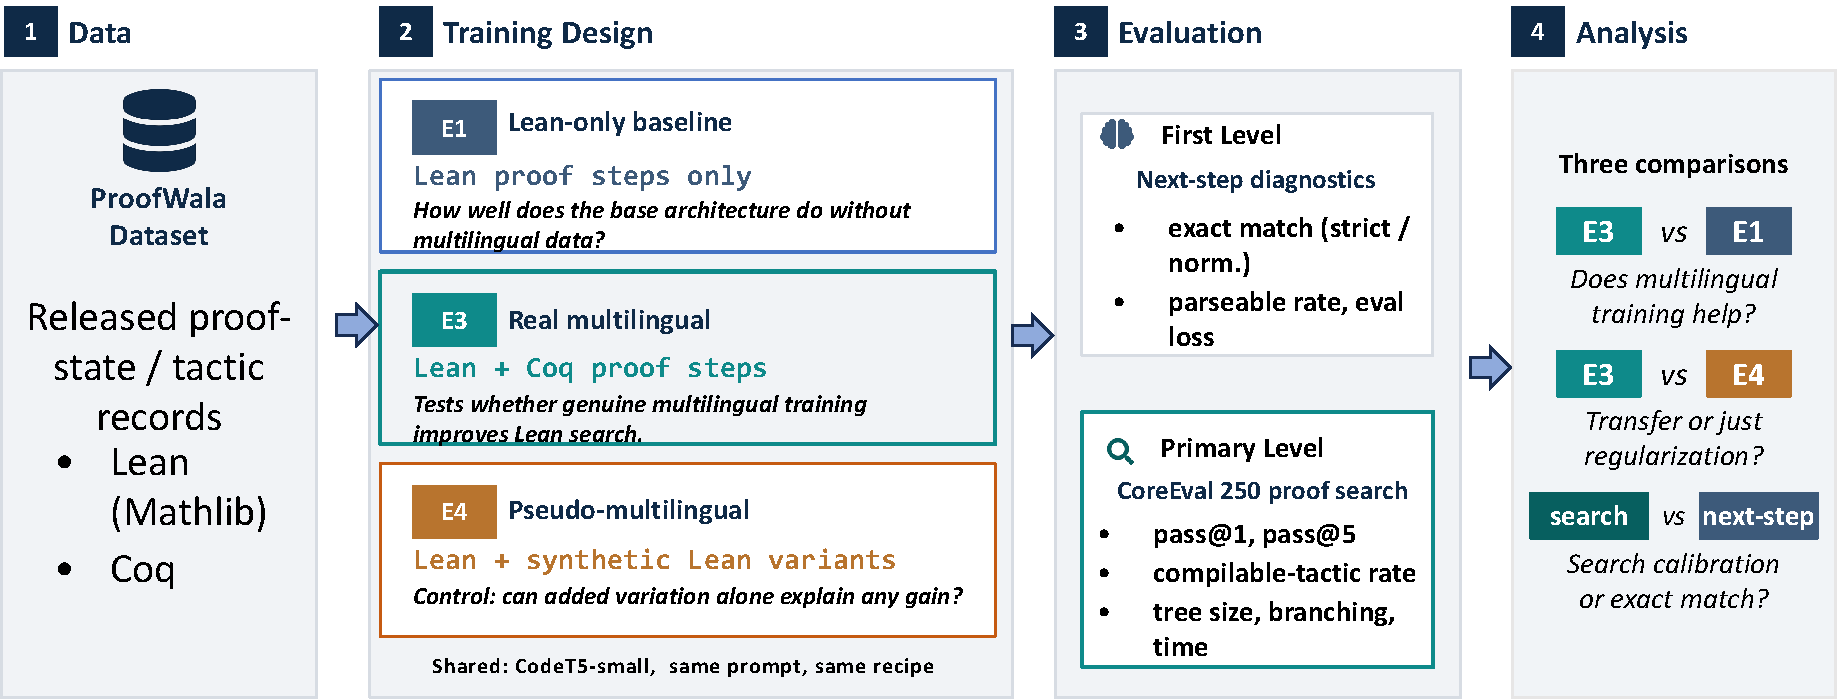
\includegraphics[width=1.0\linewidth]{Picture1.pdf}
\caption{Methodology of Three-Condition Controlled Pilot for Multilingual Theorem Proving.}
\label{fig:methodflow}
\end{figure}

\subsection{Experimental design}
\label{subsec:design}

We train three models with the same architecture and prompt format, varying
only the training data (Table~\ref{tab:experimental_design}).  This design
separates the two hypotheses: E3 tests real Lean+Rocq transfer, while E4 tests
whether syntax variation alone can explain the gain.

\begin{table}[!tbp]
\centering
\caption{Main experimental conditions.  All three trained models use the same
base model, tokenizer, prompt grammar, and Lean evaluation pipeline.}
\small
\begin{tabular}{@{}p{0.10\linewidth}p{0.24\linewidth}p{0.48\linewidth}@{}}
\toprule
\textbf{ID} & \textbf{Name} & \textbf{Purpose} \\
\midrule
E1 & Lean-only baseline & Trained only on Lean proof steps.  This model shows how well the chosen architecture performs without multilingual data. \\
E3 & Real multilingual model & Trained on ProofWala multilingual data containing Lean and Rocq proof steps.  This model tests whether real multilingual training improves Lean proof search. \\
E4 & Pseudo-multilingual control & Trained on Lean proof steps plus a synthetic Lean variant.  This model tests whether syntax variation alone can explain any gain. \\
\bottomrule
\end{tabular}
\label{tab:experimental_design}
\end{table}

If E3 beats both E1 and E4, the result favors H1.  If E4 matches or exceeds
E3, the result favors H2.  We also examine search diagnostics to see whether
differences come from more useful candidate tactics during search.

\subsection{Data sources and splits}
\label{subsec:data}

We use the released \texttt{amitayusht/ProofWalaDataset} rather than regenerating
proof-step data.  E1 uses the Lean training split.  E3 uses a project-compatible
multilingual split with Lean and Rocq examples.  E4 uses Lean data plus a
synthetic Lean variant and deliberately contains no real Rocq examples.  All
evaluation references are frozen before training and reused across E1, E3, and
E4.

\subsection{Model and training setup}
\label{subsec:training}

All three models start from \texttt{Salesforce/codet5-small}. This is a smaller, but similar model used in the ProofWala experiments (\texttt{Salesforce/codet5-base}). We chose this smaller version to reduce the training time. The input is the
serialized proof state and the output is one tactic.  We keep the same tokenizer,
prompt format, sequence lengths, and training recipe where possible.  Our final
pilot models were trained with one RTX
A5000 GPU and a 12-hour wall-time budget on the UMD Nexus cluster.


\subsection{Pseudo-multilingual control construction}
\label{subsec:e4}

We designed the E4 condition to answer a simple question: can the benefit of
multilingual training be explained by syntax variation alone?  To test
this, we augment Lean training data with synthetic Lean examples that look
syntactically different but preserve the same proof structure.  The
synthetic examples are not translated into Rocq and do not contain Rocq tactics,
Rocq lemmas, or Rocq-specific syntax.

We keep the transformation conservative.  Our script identifies local variables
and hypotheses, renames them to placeholders such as \texttt{pseudo\_0}, and
applies the same rename map to the hypotheses, goals, and target tactic.  We
avoid names with likely global meaning, such as Lean keywords, namespaces,
theorem names, constructors, tactic names, and qualified names such as
\texttt{Nat.add}.  Thus E4 changes syntax but not the proof language, task, or
prompt format.

Because synthetic data can introduce subtle errors, E4 is a pilot control rather
than a final causal control.  We audit generated examples before training and
prefer dropping risky transformations to training on invalid proof states.

\section{Evaluation}
\label{sec:evaluation}

We evaluate each model at two levels (Table~\ref{tab:evaluation_metrics}).
Next-step diagnostics ask whether the model can predict a held-out tactic from
a proof state.  Proof-search evaluation places the model inside the ProofWala
search loop~\citep{thakur2025proofwala}: the model proposes tactics, Lean checks
them, and search continues until a proof is found or the budget is exhausted.
Proof search is the primary evaluation because it measures whether the model can
finish proofs, not only imitate recorded steps.

\begin{table}[!htbp]
\centering
\small
\caption{Two-level evaluation design and metric meanings.}
\label{tab:evaluation_metrics}
\begin{tabular}{p{0.22\linewidth} p{0.24\linewidth} p{0.40\linewidth}}
\toprule
\textbf{Evaluation Level} & \textbf{Metric} & \textbf{Meaning} \\
\midrule

\multirow{4}{=}{\textbf{Next-step diagnostics}
\citep{huang2018gamepad,yang2019coqgym,blaauwbroek2020tactic}} 
& Exact match 
& Measures whether the model predicts the same next tactic as the reference proof. \\

& Normalized exact match 
& Measures tactic prediction after removing minor formatting differences. \\

& Parseable output rate 
& Measures whether the generated tactic is syntactically valid Lean code. \\

& Mean evaluation loss 
& Measures prediction error on held-out proof-step data. \\

\midrule

\multirow{5}{=}{\textbf{Proof-search evaluation} \citep{thakur2025proofwala,yang2023leandojo,lample2022hypertree}} 
& Pass@1 
& Measures whether the theorem is proved using the model's top-ranked choices. \\

& Pass@$k$ 
& Measures whether proof search succeeds after exploring up to $k$ candidate tactics. \\

& Accepted-tactic rate 
& Measures how often generated tactics are accepted by Lean during search. \\

& Early dead-end rate 
& Measures how often search stops early because no useful tactic is found. \\

& Average search time 
& Measures the computational cost of attempting each theorem. \\

\bottomrule
\end{tabular}
\end{table}

\subsection{Benchmarks and metrics}
\label{subsec:evaluation-metrics}

We evaluate the models on two Lean benchmarks.  The first is \textbf{Easy\_Lean}, a controlled set of 250 Lean problems that we constructed for this study.  The problems are relatively regular and share many proof-step patterns, so Easy\_Lean tests performance near the Lean training distribution.

The second is \textbf{Hard\_Lean}, our combined miniF2F-based external benchmark.  miniF2F is a standard theorem-proving benchmark containing formal Olympiad-level mathematics problems across proof assistants such as Lean, Metamath, Isabelle, and HOL Light~\citep{zheng2021minif2f}.  Hard\_Lean is harder and more diverse than Easy\_Lean, so it tests external generalization rather than in-project benchmark fit.

The main proof-search metric is pass rate: the fraction of attempted theorems
that are proved.  We also report accepted tactic rate, proof-tree size, branching
factor, early dead-end rate, and average search time to understand how each
model searches.

\subsection{Handling timeouts and scope of claims}
\label{subsec:evaluation-scope}

Proof search is computationally expensive, so a 12-hour Nexus job may not finish
every theorem for every model.  We therefore report both the full attempted set
and an \textit{intersection view} restricted to theorem names attempted by all
three models.

Our claims are limited to this pilot setting. The models are CodeT5-small
checkpoints trained under class-cluster storage and wall-time constraints, so
their absolute pass rates should not be interpreted as final performance numbers.
The main evidence is the relative ordering and search behavior of E1, E3, and E4
under the same model size, data-processing pipeline, benchmark, and search
budget. Because each experiment uses a single seed, we treat the results as
pilot evidence rather than statistically confirmed effects.

\section{Results and Analysis}

Table~\ref{tab:main-results} gives the main proof-search results.  We report both the full attempted set and the theorem-name intersection attempted by all three models.  The intersection view is the cleaner comparison when jobs time out at different points.

\begin{table}[H]
\centering
\caption{Proof-search results on Easy\_Lean and Hard\_Lean.  Pass rate is proved / attempted.}
\resizebox{\textwidth}{!}{
\begin{tabular}{llccccc}
\toprule
\textbf{Benchmark} & \textbf{Model} & \textbf{Attempted} & \textbf{Proved} & \textbf{Pass Rate} & \textbf{Intersection Proved} & \textbf{Intersection Pass Rate} \\
\midrule
\multirow{3}{*}{Easy\_Lean} 
& E1: Lean-only & 127 & 49 & 38.6\% & 49 & 38.6\% \\
& E3: Real multilingual & 141 & 43 & 30.5\% & 39 & 30.7\% \\
& E4: Pseudo-multilingual & 198 & 126 & 63.6\% & 78 & 61.4\% \\
\midrule
\multirow{3}{*}{Hard\_Lean}
& E1: Lean-only & 77 & 2 & 2.6\% & 2 & 2.6\% \\
& E3: Real multilingual & 81 & 4 & 4.9\% & 4 & 5.2\% \\
& E4: Pseudo-multilingual & 87 & 3 & 3.4\% & 3 & 3.9\% \\
\bottomrule
\end{tabular}
}
\label{tab:main-results}
\end{table}

The results are distribution-dependent.  On Easy\_Lean, E4 is the clear winner: it proves 126 theorems overall and 78 on the shared intersection, compared with 49 for E1 and 39 for E3.  The Easy\_Lean result was unexpected and surprising for two reasons.  First, ProofWala suggests that real multilingual training should improve over a Lean-only baseline, but E3 is below E1 here.  Second, E4 improves by a large margin over both E1 and E3.  This supports the regularization hypothesis, but we do not yet understand why the improvement is so strong; explaining its size requires further experiments and a more careful audit of the pseudo-Lean transformation.

Hard\_Lean changes the ordering.  E3 proves 4 theorems, compared with 3 for E4 and 2 for E1.  The pass rates are low because Hard\_Lean is timeout-heavy, but the ordering matters: real multilingual training is strongest on the harder external benchmark, while E1 and E4 become much closer than on Easy\_Lean.

\begin{table}[H]
\centering
\caption{Search diagnostics.  Accepted action rate is parser/action acceptance during proof search, not a standalone proof-correctness metric.}
\resizebox{\textwidth}{!}{
\begin{tabular}{llcccccc}
\toprule
\textbf{Benchmark} & \textbf{Model} & \textbf{Valid Tactics / State} & \textbf{Accepted Rate} & \textbf{Early Dead-End} & \textbf{Mean Nodes} & \textbf{Mean Branching} & \textbf{Mean Time (s)} \\
\midrule
\multirow{3}{*}{Easy\_Lean}
& E1 & 12.060 & 1.000 & 0.000 & 3.141 & 4.164 & 231.338 \\
& E3 & 12.840 & 1.000 & 0.000 & 2.915 & 3.258 & 195.715 \\
& E4 & 12.789 & 1.000 & 0.000 & 3.232 & 3.929 & 150.511 \\
\midrule
\multirow{3}{*}{Hard\_Lean}
& E1 & 11.358 & 1.000 & 0.000 & 2.117 & 2.137 & 490.195 \\
& E3 & 12.941 & 1.000 & 0.000 & 2.185 & 1.981 & 456.315 \\
& E4 & 11.781 & 1.000 & 0.000 & 2.195 & 2.298 & 405.301 \\
\bottomrule
\end{tabular}
}
\label{tab:search-diagnostics}
\end{table}

The search diagnostics reinforce the main story.  E4 is fastest on both benchmarks, which helps explain its Easy\_Lean throughput.  E3 generates the most valid tactics per state on Hard\_Lean and solves the most Hard\_Lean theorems, suggesting that its benefit appears most clearly on the harder external distribution.

\begin{table}[H]
\centering
\caption{Hard\_Lean theorems proved by each model.}
\small
\begin{tabular}{llcc}
\toprule
\textbf{Model} & \textbf{Theorem} & \textbf{Time (s)} & \textbf{Tactic} \\
\midrule
E1 & \texttt{mathd\_numbertheory\_342} & 122.1 & \texttt{norm\_num1} \\
E1 & \texttt{mathd\_algebra\_176} & 57.4 & \texttt{ring} \\
E3 & \texttt{amc12b\_2020\_p2} & 114.8 & \texttt{ring1} \\
E3 & \texttt{mathd\_numbertheory\_207} & 100.7 & \texttt{norm\_num} \\
E3 & \texttt{mathd\_algebra\_329} & 68.6 & \texttt{linarith} \\
E3 & \texttt{mathd\_algebra\_176} & 85.7 & \texttt{ring} \\
E4 & \texttt{mathd\_numbertheory\_207} & 114.6 & \texttt{ring} \\
E4 & \texttt{mathd\_algebra\_176} & 86.2 & \texttt{ring1} \\
E4 & \texttt{mathd\_numbertheory\_175} & 92.1 & \texttt{norm\_num} \\
\bottomrule
\end{tabular}
\label{tab:hard-lean-proved}
\end{table}

The overlap is also informative.  All three models prove \texttt{mathd\_algebra\_176}; E3 and E4 both prove \texttt{mathd\_numbertheory\_207}; and each model has at least one unique success.  Thus Hard\_Lean does not merely repeat the Easy\_Lean ranking.

\subsection{Interpretation and Limitations}

The strongest conclusion is not that one training method is always best.  The mechanism depends on the theorem distribution.  Easy\_Lean supports H2: syntax variation improves Lean-like proof search.  Hard\_Lean gives weaker but useful support for H1: real multilingual training can help on harder external theorem styles.

Several limitations qualify these claims.  E3 used a practical multilingual split rather than a perfectly token-matched Lean+Rocq mixture.  E4's pseudo-Lean transformation is conservative but still requires further auditing.  Hard\_Lean has low proof counts, so its ordering should be treated as pilot evidence.  Finally, all experiments use one model size, one seed, and Nexus class-cluster time and storage constraints.  Figure~\ref{fig:overview-results} summarizes the final interpretation.

\begin{figure}[H]
\centering
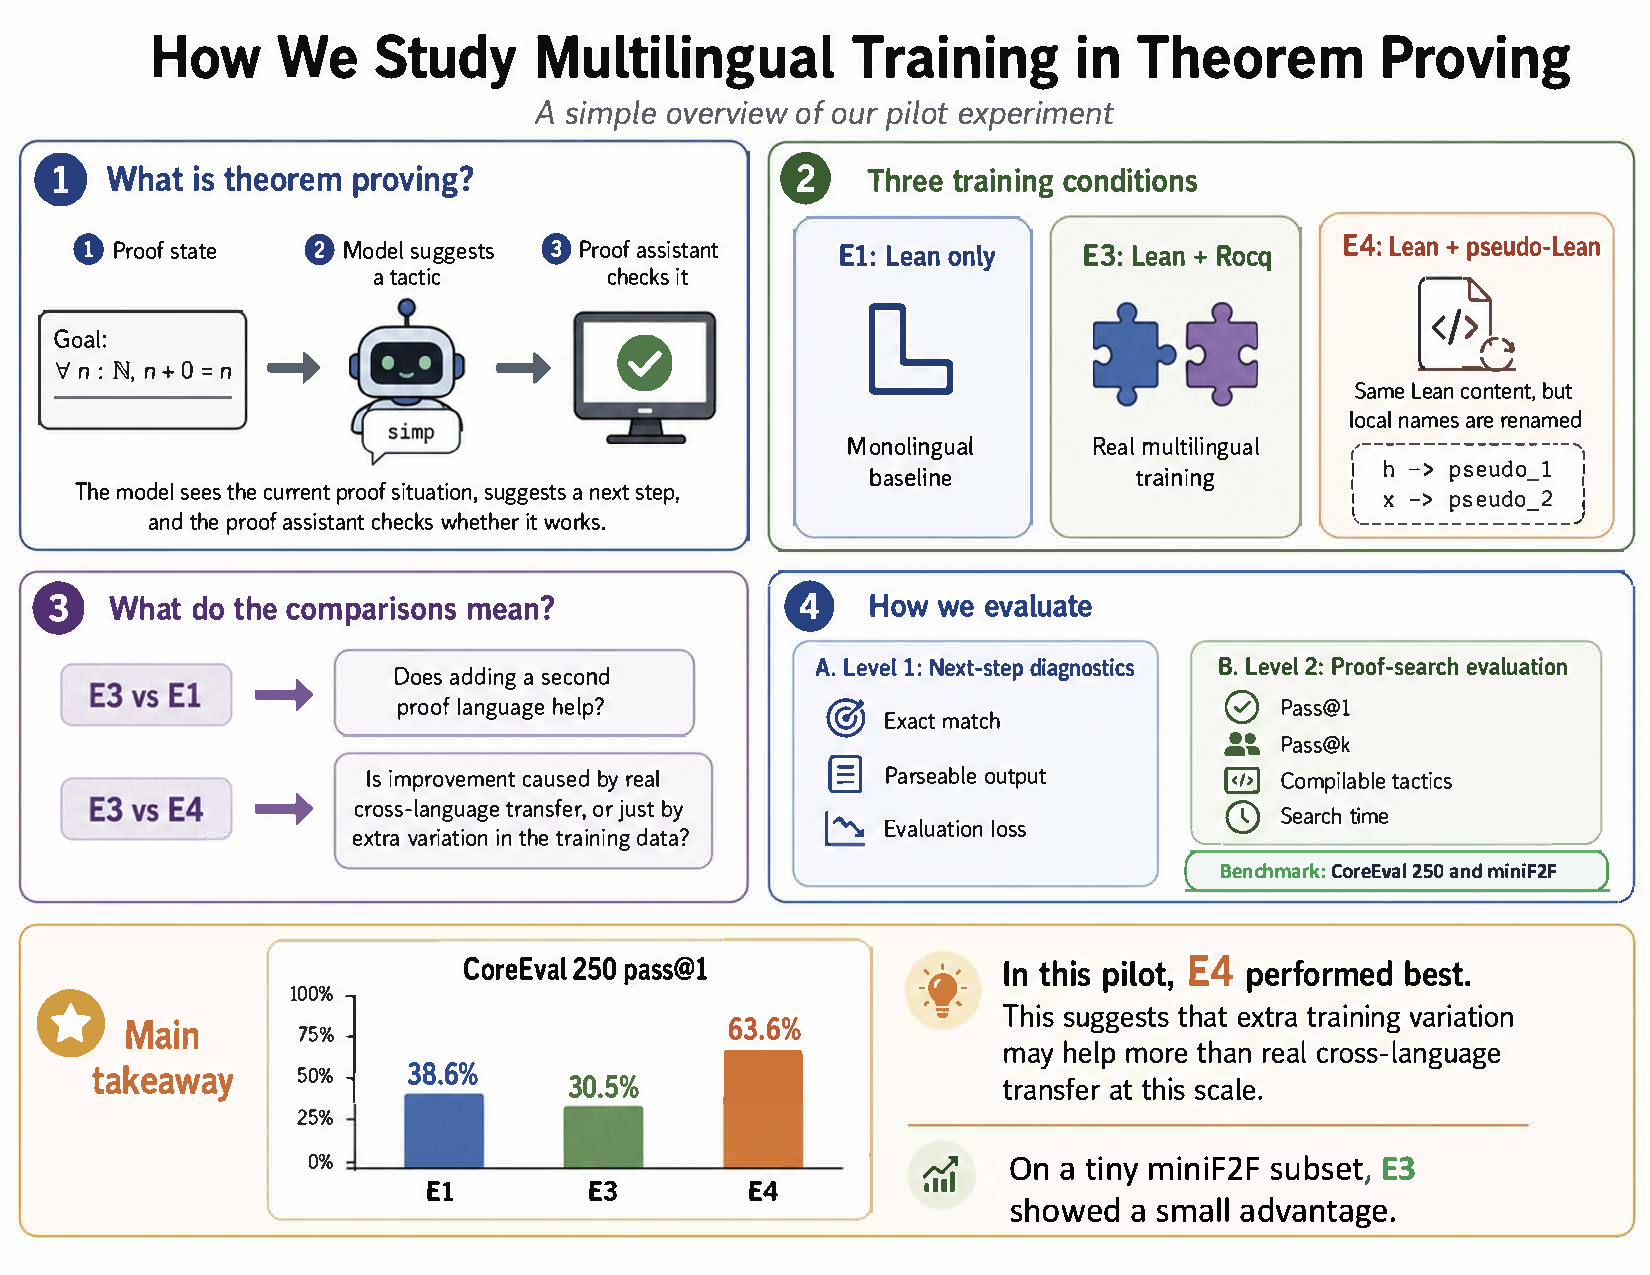
\includegraphics[width=0.95\linewidth]{overall view of project.pdf}
\caption{Summary of the main result: Easy\_Lean favors pseudo-multilingual regularization, while Hard\_Lean gives the strongest result to real multilingual training.}
\label{fig:overview-results}
\end{figure}

\section{Data, Code, and Reproducibility}
\label{subsec:Data, Code, and Reproducibility}

All code, configs, and frozen data splits are available at
\url{https://github.com/AmadeoDeLaVega/multilingual-project}.
The repository contains the ProofWala and ITP-interface code, Hydra training
configs for E1/E3/E4, frozen split references, SLURM scripts under
\texttt{scripts/nexus/}, and the copied evaluation outputs that produced
Table~\ref{tab:main-results}.
The \texttt{Salesforce/codet5-small} base weights are downloaded from
Hugging Face at install time and are not bundled; the Nexus SLURM
scripts assume the UMIACS \texttt{class} partition and will need
adaptation for other clusters.
Each training run used one NVIDIA A5000 GPU with a 12-hour wall-time budget.
Proof-search evaluation was also run through SLURM and may stop by wall-time,
which is why we report both attempted-theorem counts and intersection results.
Re-running with the same configs and seed~42 should reproduce
Table~\ref{tab:main-results} up to normal CUDA and cluster nondeterminism.
See \texttt{README.md} for step-by-step setup instructions.


\section{Statement of Contributions}
\label{sec:contributions}

Amadeo De La Vega led the development of the project, the implementation of the training and proof-search pipeline, ran the main Nexus jobs, managed result collection, and revised the report and presentation.  Mehak Gupta contributed to code review and Nexus testing, helped write the problem statement, related work, and results discussion, and prepared the presentation slides.  Huan Zhou contributed to code review and Nexus testing and helped write the methodology and evaluation-design sections.  All authors discussed the experimental framing and interpretation.


 



\bibliography{colm2026_conference}
\bibliographystyle{colm2026_conference}

\end{document}
